In Guatemala the site is located at the top of the roof of the T1 building of the University of San Carlos de Guatemala (an altitude of 1490 m). The size of the detector is 1.2\,m height, 1.12\,m wide and has a capacity of 1,100\,lts. It is filled with comercial demineralized water and the inside is coated with a reflective Flex polyvinyl chloride sheet. The Cherenkov photons are recolected with a 9" Photonis XP1802 PMT.  

The electronics of the detector, original from the Bariloche group, was repaired after an approximately a year of functioning. Later, the visit of Ruben Conde from the Astroparticle group of the University of Puebla, initiated the development of a new electronic system. The purification process of water is not yet implemented and currently the detector is on hold because of the above reasons. 

\begin{figure}[h]

\begin{center}

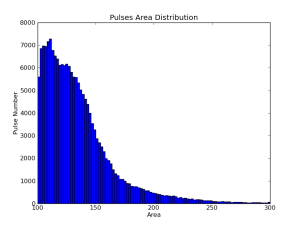
\includegraphics[width=\textwidth]{Histo.png}

\caption{Histogram of an event of the uncalibrated detector. The area is proportional to the charge recolected. The second peak corresponds to a muonic trace.

\label{fig:Histo-guate} 

\end{center}

\end{figure}

\begin{figure}[h]

\begin{center}

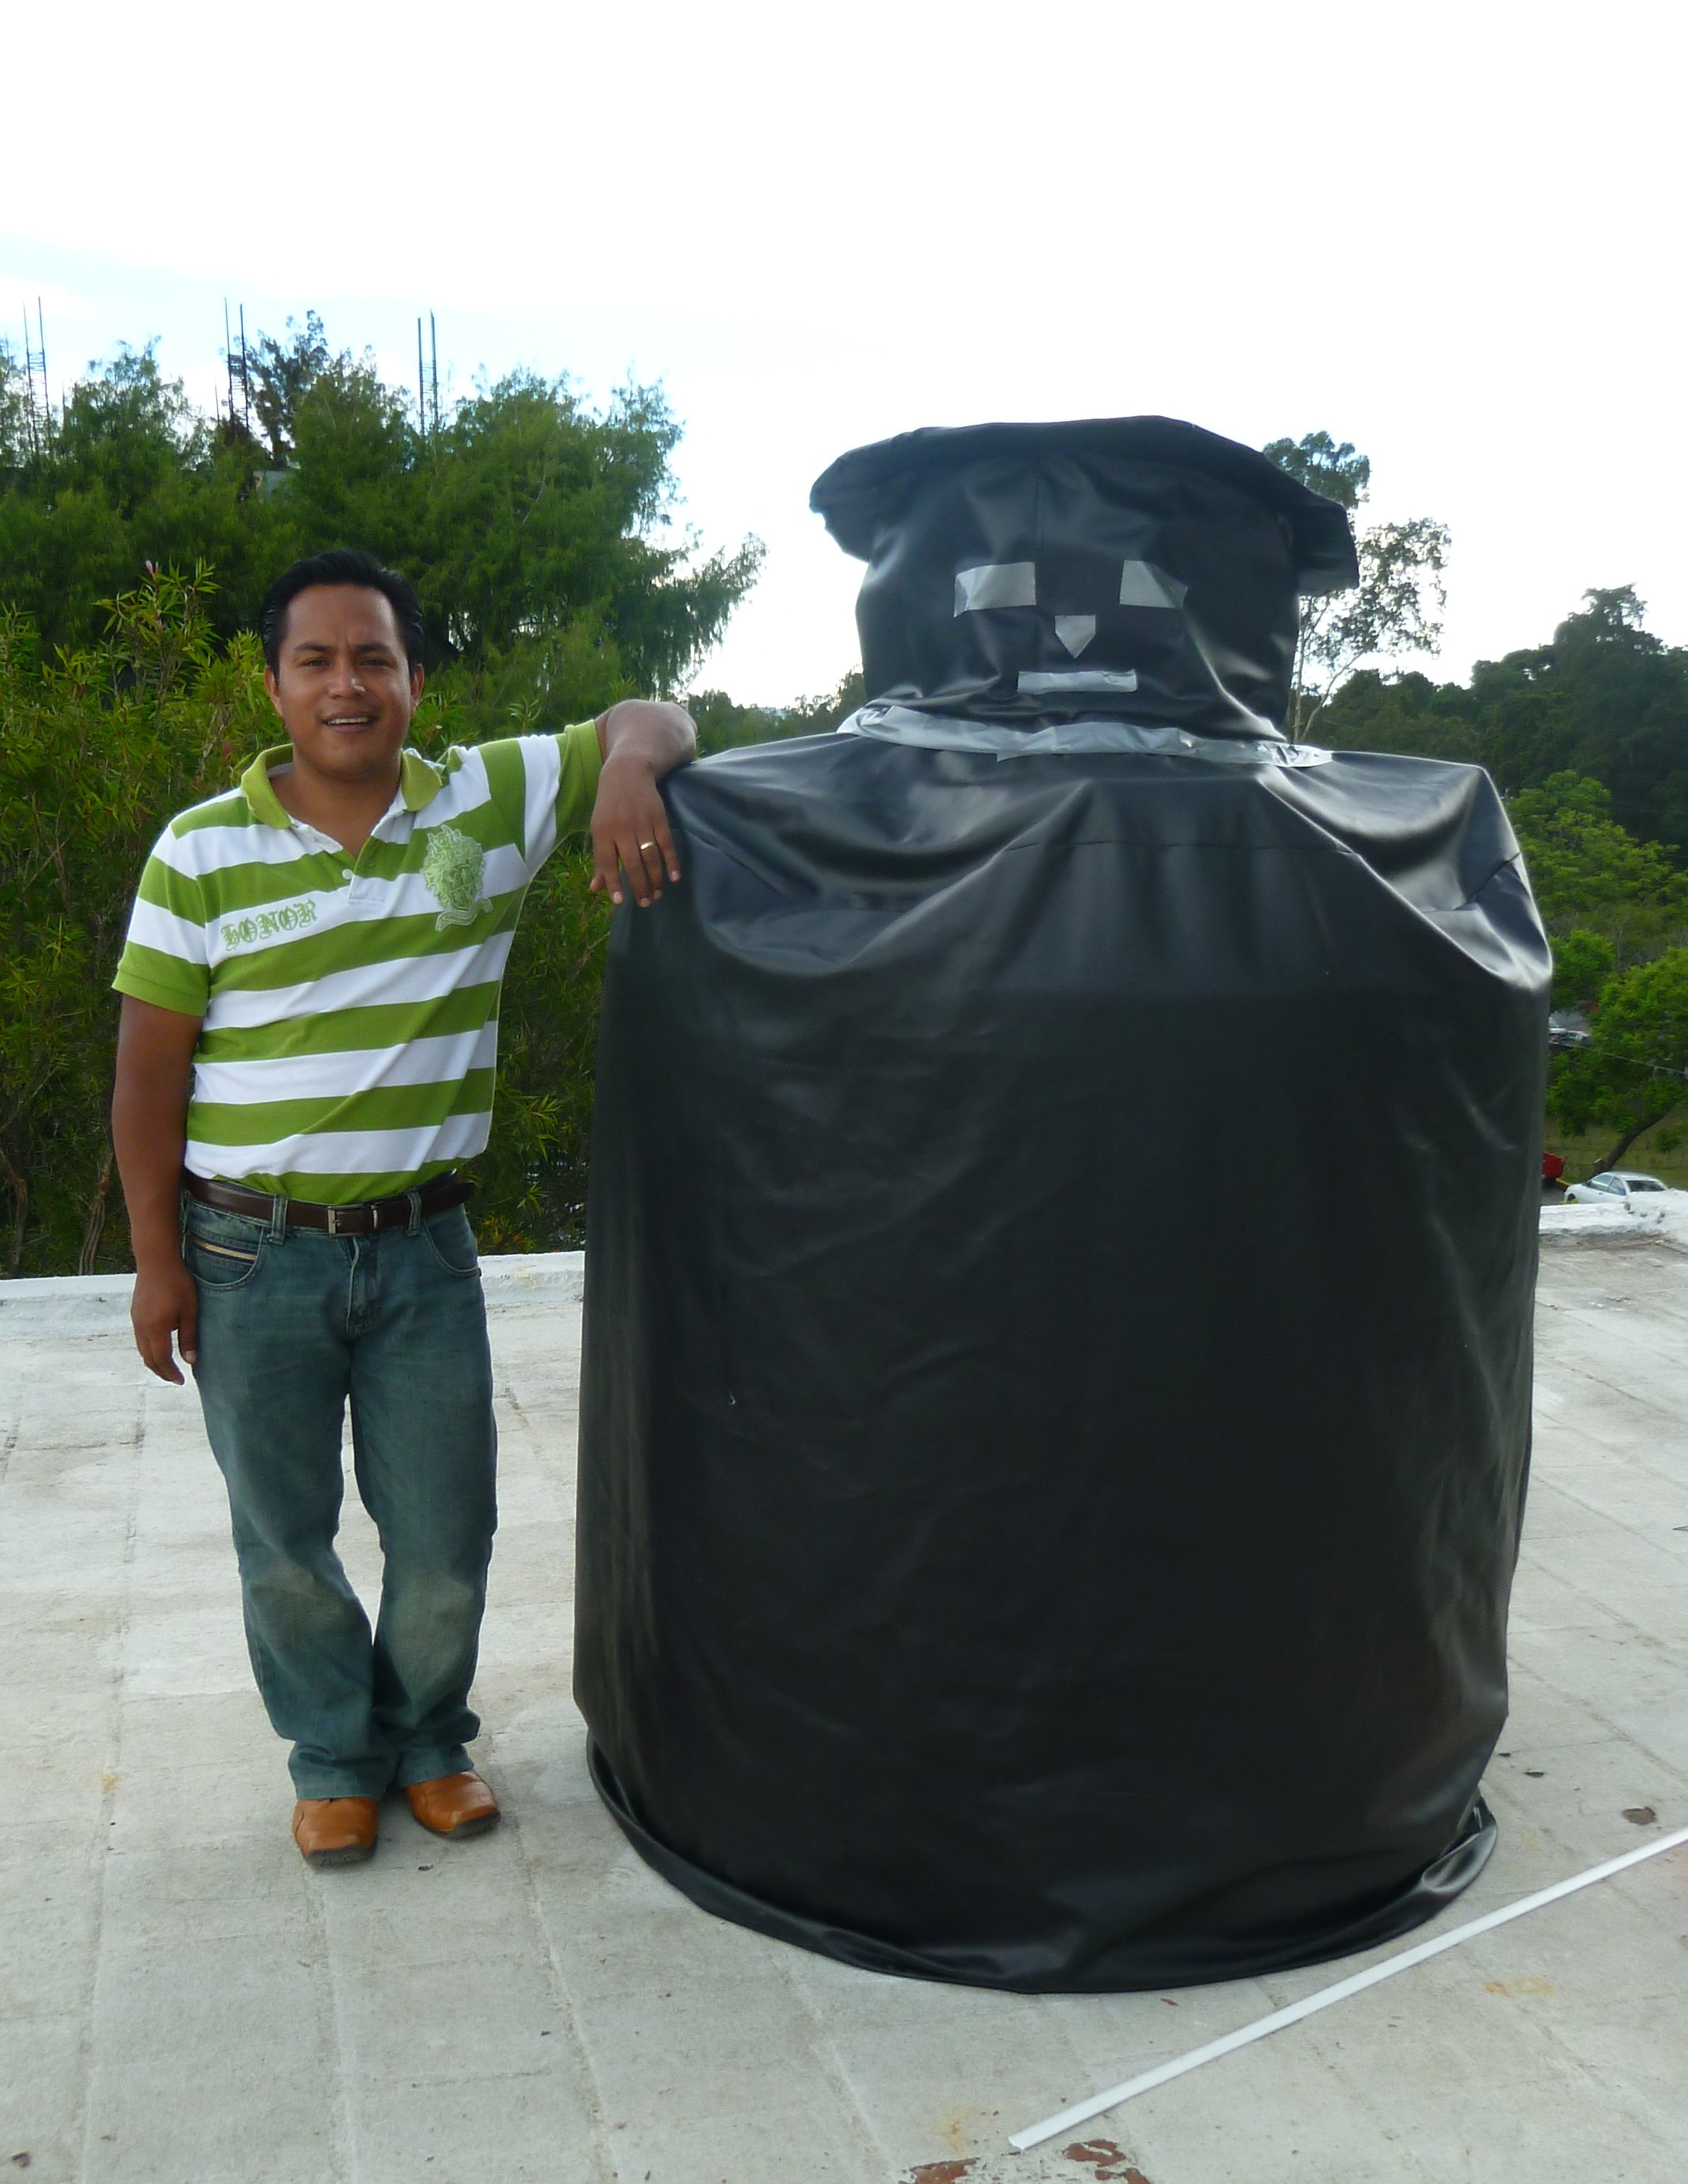
\includegraphics[width=\textwidth]{DimDet.jpg}

\caption{The entire detector is covered with black semi-leather. }

\label{fig:guate-tanque} 

\end{center}

\end{figure} 
